\documentclass[11pt,oneside,a4paper]{book}
% Paquetes basicos cargados al inicio
\usepackage[utf8]{inputenc}
\usepackage{graphicx}
\usepackage{lmodern}
\usepackage[a4paper,top=2.54cm,bottom=2.0cm,left=2.0cm,right=2.54cm]{geometry} % margenes
\usepackage{amsmath,amsfonts,amssymb,amscd,amsthm,xspace}
\theoremstyle{plain}
\newtheorem{example}{Example}[chapter]
\newtheorem{theorem}{Theorem}[chapter]
\newtheorem{corollary}{Corollary}[chapter]
\newtheorem{lemma}{Lemma}[chapter]
\newtheorem{proposition}{Proposition}[chapter]
\newtheorem{axiom}{Axiom}[chapter]
\theoremstyle{definition}
\newtheorem{definition}{Definition}[chapter]
\newtheorem{assumption}{Assumption}
\renewcommand\theassumption{A\arabic{assumption}}

% Paquetes adicionales
\usepackage{natbib} % Bibliografia
\usepackage{lipsum} % Generar lero leros
\usepackage{setspace} % Para modificar el espaciio entre lineas
\setstretch{1.6} 
\usepackage{indentfirst} % Indentação do primeiro parágrafo

\usepackage{afterpage}

\newcommand\blankpage{%
    \null
    \thispagestyle{empty}%
    \addtocounter{page}{-1}%
    \newpage
}

\usepackage{multirow}
\usepackage{float}

\usepackage{url}

% Show line numbers
\usepackage[mathlines]{lineno}
\renewcommand\linenumberfont{\normalfont\small\color{gray}}

% Show labels
% \usepackage{showlabels}

\newcommand{\R}{\mathbb{R}}
\newcommand{\N}{\mathbb{N}}
\newcommand{\xtrial}{x^{\mathrm{trial}}}
\newcommand{\ytrial}{y^{\mathrm{trial}}}
\newcommand{\flow}{f_{\mathrm{low}}}
\newcommand{\Flow}{F_{\mathrm{low}}}
\newcommand{\Fmin}{F_{\mathrm{min}}}
\newcommand{\Imin}{I_{\mathrm{min}}}
\newcommand{\Imax}{I_{\mathrm{max}}}
\newcommand{\Pcal}{\mathcal{P}}

\DeclareMathOperator*{\Minimize}{Minimize}
\DeclareMathOperator*{\co}{co}
\DeclareMathOperator*{\inter}{int}

\usepackage{fancyhdr}
\usepackage{caption}
\usepackage{subcaption}

% %Estilo algoritmo Gustavo
\usepackage{enumitem} % Essencial pro estilo algoritmo gustavo (enumera os passos)
\setlist[enumerate,1]{itemindent=2em}
\setlist[enumerate,2]{itemindent=3em}
\newcounter{counter}
\counterwithin{counter}{chapter}
\newcommand{\algorithm}[3]{
\refstepcounter{counter}
\label{#1}
{\noindent\bf Algorithm~\thecounter:} #2
\vspace{-1.3\topsep}
\begin{enumerate}[leftmargin=2.5\parindent]
\renewcommand{\labelenumi}{\textbf{\theenumi}.}
\renewcommand{\labelenumii}{\textbf{\theenumii}.}

\renewcommand{\theenumi}{Step~\arabic{enumi}}
\renewcommand{\theenumii}{Step~\arabic{enumi}.\arabic{enumii}}

\setlength{\itemsep}{1ex}
\setlength{\parskip}{0pt}
\setlength{\parsep}{0pt}
#3
\end{enumerate}
}
\usepackage[usenames,svgnames,dvipsnames]{xcolor}% Para nuevos colores: DarkGreen, NavyBlue, DarkRed

\usepackage[pdftex,plainpages=false,pdfpagelabels,pagebackref,colorlinks=true,citecolor=DarkGreen,linkcolor=NavyBlue,urlcolor=DarkRed,filecolor=green,bookmarksopen=true]{hyperref} % links coloridos

\newcommand{\autor}{Name of the work's author}
\newcommand{\tituloen}{English title}
\newcommand{\titulopt}{Título em Portugués}
\newcommand{\orientador}{Prof. Dr. Advisor name}
\newcommand{\coorientador}{Prof. Dr. Co-advisor name}

\begin{document}
\fancyhead{} % Clears all page headers and footers
\rhead{\thepage} % Sets the right side header to show the page number
\lhead{} % Clears the left side page header

\pagestyle{fancy} % The page style headers have been "empty" all this time, now use the "fancy" headers as defined before to bring them back

\renewcommand{\backrefpagesname}{Cited in page(s):~}
% Texto padrão antes do número das páginas
\renewcommand{\backref}{}
% Define os textos da citacao
\renewcommand*{\backrefalt}[4]{
	\ifcase #1 %
		No citations in the text.%
	\or
		Cited on page #2.%
	\else
		Cited #1 times on pages #2.%
	\fi}%
% ---
% TIPO DE TRABALHOS
% Copiar e colar na parte "Tipo de trabalho" da capa

% Qualificação:

%RELATÓRIO APRESENTADO AO\\
%INSTITUTO DE MATEMÁTICA E ESTATÍSTICA\\
%DA UNIVERSIDADE DE SÃO PAULO\\
%PARA EXAME DE QUALIFICAÇÃO DE\\
%DOUTOR(A) EM CIÊNCIAS

% Dissertação:

%DISSERTAÇÃO APRESENTADA AO\\
%INSTITUTO DE MATEMÁTICA E ESTATÍSTICA\\
%DA UNIVERSIDADE DE SÃO PAULO\\
%PARA OBTENÇÃO DO TÍTULO DE\\
%MESTRE(A) EM CIÊNCIAS

% Tese:

%TESE APRESENTADA AO\\
%INSTITUTO DE MATEMÁTICA E ESTATÍSTICA\\
%DA UNIVERSIDADE DE SÃO PAULO\\
%PARA OBTENÇÃO DO TÍTULO DE\\
%DOUTOR(A) EM CIÊNCIAS

% APOIO
% Copiar e colar na parte "Tipo de apoio" da capa
% Norma sobre agradecimento por auxílios da FAPESP:
% https://fapesp.br/11789/referencia-ao-apoio-da-fapesp-em-todas-as-		formas-de-divulgacao
%
% Norma sobre agradecimento por auxílios da CAPES (Portaria 206,
% de 4 de Setembro de 2018):
% https://www.in.gov.br/materia/-/asset_publisher/Kujrw0TZC2Mb/content/id/39729251/do1-2018-09-05-portaria-n-206-de-4-de-setembro-de-2018-39729135

% Apoio (CAPES):

% O presente trabalho foi realizado com apoio da Coordenação
%       de Aperfeiçoamento\\ de Pessoal de Nível Superior -- Brasil
%       (CAPES) -- Código de Financiamento 001}, % o código é sempre 001
%
% This study was financed in part by the Coordenação de
%       Aperfeiçoamento\\ de Pessoal de Nível Superior -- Brasil
%       (CAPES) -- Finance Code 001, % o código é sempre 001

% Apoio (FAPESP):

% Durante o desenvolvimento deste trabalho, o autor recebeu\\
%       auxílio financeiro da FAPESP -- processo nº aaaa/nnnnn-d,
%
% During the development if this work, the author received\\
%       financial support from FAPESP -- grant \#aaaa/nnnnn-d,

% Capa
\begin{titlepage}
\begin{center}
\begin{minipage}[t][56mm][s]{96mm}
          \vspace*{2cm plus 1.5cm minus 1.8cm}

          \centering

          {\Large \bfseries\tituloen}\\[0.4cm] % Thesis title

          \vspace{1cm plus 1cm minus 0.6cm}

          {\Large\autor}

          \vspace*{2cm plus 1.5cm minus 1.8cm}
      \end{minipage}

\vfill
% Dissertação:


% Tipo de trabalho
    \textsc{\large{
    REPORT PRESENTED TO THE\\
    INSTITUTE OF MATHEMATICS AND STATISTICS\\
    OF THE UNIVERSITY OF SÃO PAULO\\
    FOR THE DOCTOR OF SCIENCE\\
    QUALIFYING EXAMINATION}}
    
    \vskip 1.5cm
    \large{
    Program: Applied Mathematics\\
    Advisor: \orientador\\
    Co-advisor: \coorientador}

   	\vfill
   	% Apoio
    \normalsize{This study was financed in part by the Coordenação de
         Aperfeiçoamento\\ de Pessoal de Nível Superior -- Brasil
         (CAPES) -- Finance Code 001}
    
    \vskip 1.5cm
    \normalsize{São Paulo, Brasil}\\
    \normalsize{August 2022}
\end{center}
\end{titlepage}

\newpage
% Para a folha de rosto copiar segundo o tipo de trabalho na parte "Texto folha de rosto" abaixo.

% Qualificação:

%This is the original version of the qualifying text
%prepared by candidate \autor,
%as submitted to the Examining Committee.

%Esta é a versão original do texto de qualificação elaborado pelo(a) candidato(a) \autor, 
%tal como submetido à Comissão Julgadora.

% Dissertação:

%This is the original version of the master thesis prepared
%by candidate \autor, as submitted to the Examining Committee.

%Esta é a versão original da dissertação elaborada pelo(a) candidato(a) \autor, tal como submetida à Comissão Julgadora.

% Tese:

%This is the original version of the thesis prepared
%by candidate \autor, as submitted to the Examining Committee.

%Esta é a versão original da tese elaborada pelo(a) candidato(a) \autor, tal como submetida à Comissão Julgadora.

%Folha de rosto
\thispagestyle{empty}
    \begin{center}
 \begin{minipage}[t][56mm][s]{96mm}
          \vspace*{2cm plus 1.5cm minus 1.8cm}
          \centering
          {\Large \bfseries \tituloen}\\[0.4cm]
           \vspace{1cm plus 1cm minus 0.6cm}

           {\Large\autor}

          \vspace*{2cm plus 1.5cm minus 1.8cm}
      \end{minipage}
     \end{center}
\vskip 2cm
\setstretch{1.3}
   \begin{flushright}
      \begin{minipage}[t][50mm][s]{80mm}
        \begin{flushright}
        % Texto folha de rosto
          \normalsize{
          This is the original version of the qualifying text
          prepared by candidate \autor,
          as submitted to the Examining Committee. 
          }
        \end{flushright}
        \vspace*{0pt plus 50mm}
      \end{minipage}
      \par
    %} % fbox
  \end{flushright}

\afterpage{\blankpage}

% Agradecimentos
\clearpage 
\thispagestyle{plain}
\pagenumbering{roman} 
\begin{center}{\huge{\textit{Acknowledgements}} \par}\end{center}
\vspace{1em}
\lipsum[1]
\lipsum[1]
\vfil\vfil\null

% SE A LÍNGUA FOR PORTGUÊS COLOCAR O ABSTRACT ANTES DO RESUMO. SE FOR EM INGLÊS DEIXA COMO ESTÁ

% Resumo
\afterpage{\blankpage}
\clearpage % Start a new page
 \thispagestyle{empty}
  %\null\vfil
  \begin{flushleft}
    \setlength{\parskip}{0pt}
    {\centering{\huge{\textit{Resumo}}} \par} 
    \bigskip
		\begin{center}
\noindent\begin{minipage}{0.75\textwidth}
\small{\autor. {\bfseries\titulopt}. 
Exame de Qualificação (Doutorado) - Instituto de Matemática e Estatística,
Universidade de São Paulo, São Paulo, 2022.}
\end{minipage}
\end{center}
\end{flushleft}
\bigskip
\lipsum[1]

% Abstract
\afterpage{\blankpage}
\clearpage % Start a new page
\thispagestyle{empty}
  %\null\vfil
  \begin{flushleft}
    \setlength{\parskip}{0pt}
    {\centering{\huge{\textit{Abstract}}} \par} 
    \bigskip
		\begin{center}
\noindent\begin{minipage}{0.75\textwidth}
\small{\autor. \textbf\tituloen. 
Qualifying Exam (Doctorate) - Institute of Matemathics and Statistics,
University of São Paulo, São Paulo, 2022.}
\end{minipage}
\end{center}
\end{flushleft}
\bigskip
\lipsum[1]

% Sumario
\lhead{\emph{Contents}} % Set the left side page header to "Contents"
\let\cleardoublepage\clearpage
\tableofcontents

% Lista de figuras
\lhead{\emph{List of Figures}} % Set the left side page header to "List of Figures"
\listoffigures % Write out the List of Figures
\addcontentsline{toc}{chapter}{List of Figures}

% Lista de tabelas
\lhead{\emph{List of Tables}} % Set the left side page header to "List of Tables"
\listoftables % Write out the List of Tables
\addcontentsline{toc}{chapter}{List of Tables}

\setstretch{1.5} % Set the line spacing to 1.5, this makes the following tables easier to read

% Lista de abreviacoes
\lhead{\emph{Abbreviations}} % Set the left side page header to "Abbreviations"
\chapter*{Abbreviations}
\addcontentsline{toc}{chapter}{Abbreviations}

% Lista de simbolos
\lhead{\emph{Symbols}} % Set the left side page header to "Symbols"
\chapter*{List of Symbols}
\begin{tabular}{ll}
        $\omega$    & Frequência angular\\
        $\psi$      & Função de análise \emph{wavelet}\\
        $\Psi$      & Transformada de Fourier de $\psi$\\
\end{tabular}
\addcontentsline{toc}{chapter}{List of Symbols}

% Dedicatoria
\clearpage
\thispagestyle{empty}
\setstretch{1.3} % Return the line spacing back to 1.3
\pagestyle{empty} % Page style needs to be empty for this page
\vspace*{\fill}
\begin{center}
{\Large\it to my parents}
\end{center}
\vspace*{\fill}

\mainmatter % Begin numeric (1,2,3...) page numbering
\pagestyle{fancy}
\setlength{\parskip}{0.5\baselineskip} % Set space between paragraphs
% Conteudo
\linenumbers
% Chapter Template

\chapter{Introduction} % Main chapter title

\label{Chapter1}

\lhead{Chapter 1. \emph{Introduction}} % Change X to a consecutive number; this is for the header on each page - perhaps a shortened title
\lipsum[1]\\
\lipsum[1]\\
\lipsum[1]

Figure~\ref{fig:ovexamples} below represents each of the situations given in the previous examples, for different values of $J$. Given 4 functions (a), the black functions in (b), (c) and (d), represent the Order-Value functions for the Min-min, Min-max and VaR-like problems, respectively. 
\begin{figure}[H]
     \centering
     \begin{subfigure}{0.32\textwidth}
         \centering
         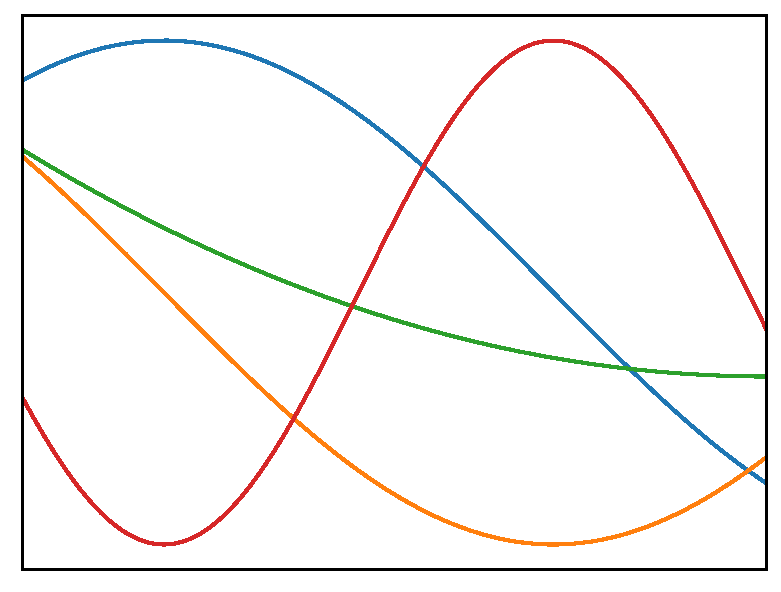
\includegraphics[width=\textwidth]{pictures/scenarios.pdf}
         \caption{$m=4$}
         \label{fig:scenarios}
     \end{subfigure}
     \hfill
     \begin{subfigure}{0.32\textwidth}
         \centering
         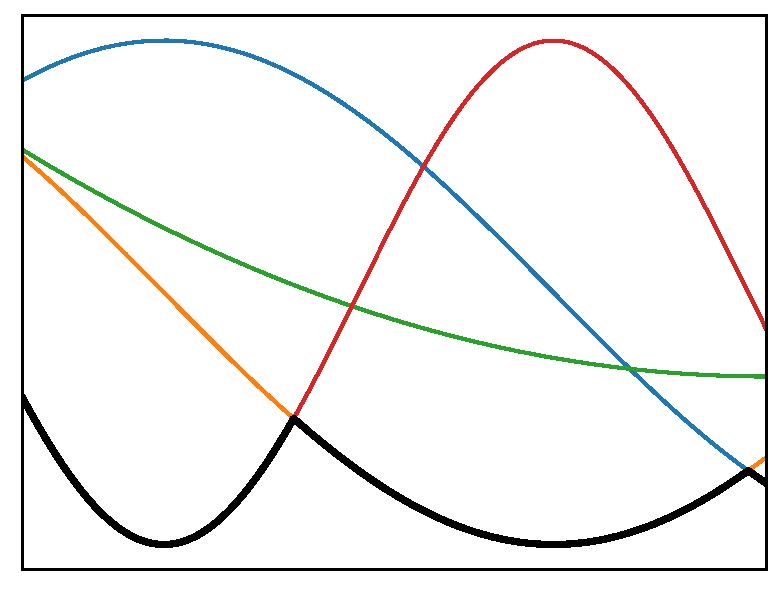
\includegraphics[width=\textwidth]{pictures/minimin.pdf}
         \caption{$J=\{1\}$}
         \label{fig:minimin}
     \end{subfigure}
     \hfill
     \begin{subfigure}{0.32\textwidth}
         \centering
         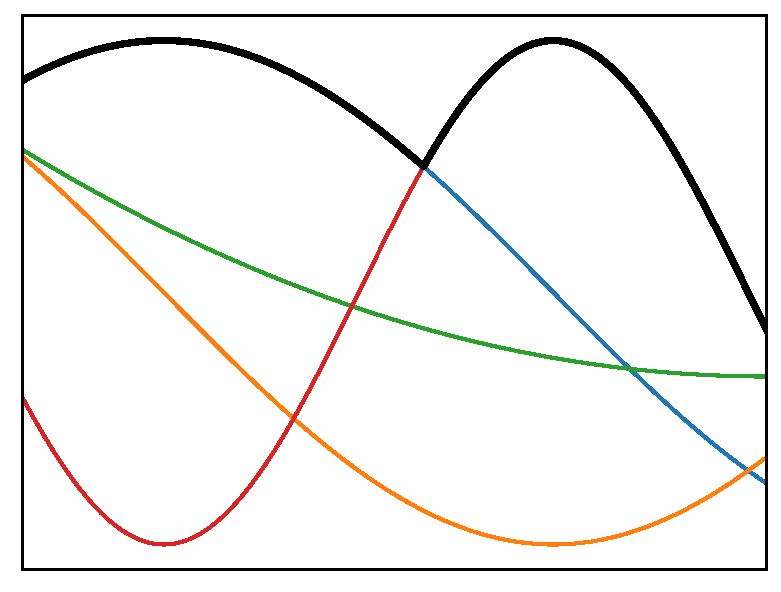
\includegraphics[width=\textwidth]{pictures/minimax.pdf}
         \caption{$J=\{4\}$}
         \label{fig:minimax}
     \end{subfigure}

     \begin{subfigure}{0.32\textwidth}
         \centering
         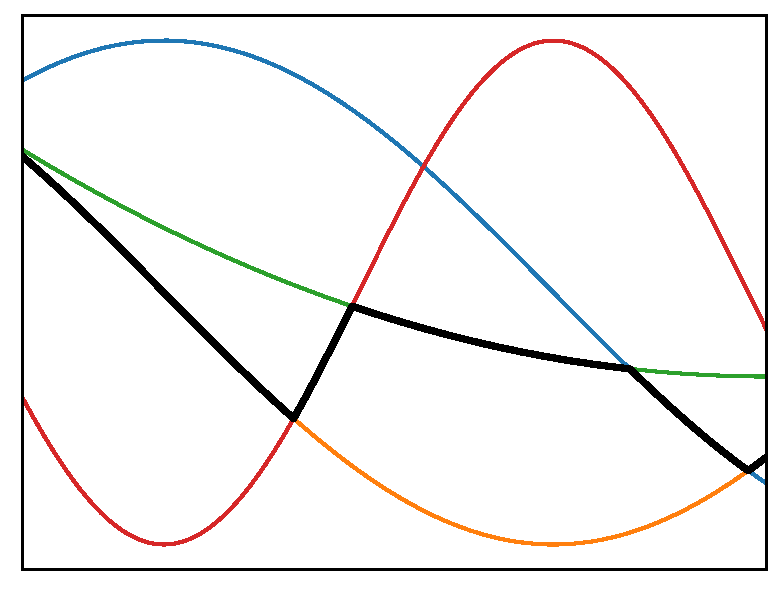
\includegraphics[width=\textwidth]{pictures/var.pdf}
         \caption{$J=\{2\}$}
         \label{fig:var}
     \end{subfigure}
     \hfill
     \begin{subfigure}{0.32\textwidth}
         \centering
         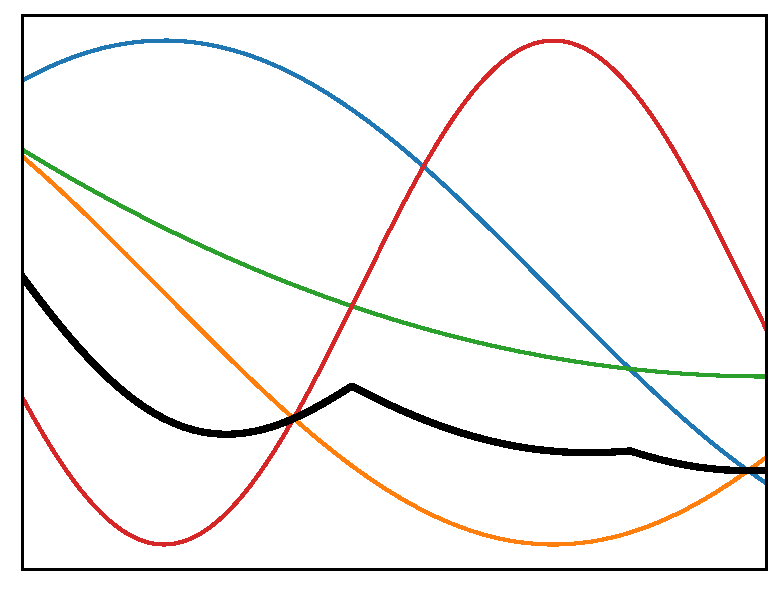
\includegraphics[width=\textwidth]{pictures/lovo.pdf}
         \caption{$J=\{1,2\}$}
         \label{fig:lovo}
     \end{subfigure}
     \hfill
     \begin{subfigure}{0.32\textwidth}
         \centering
         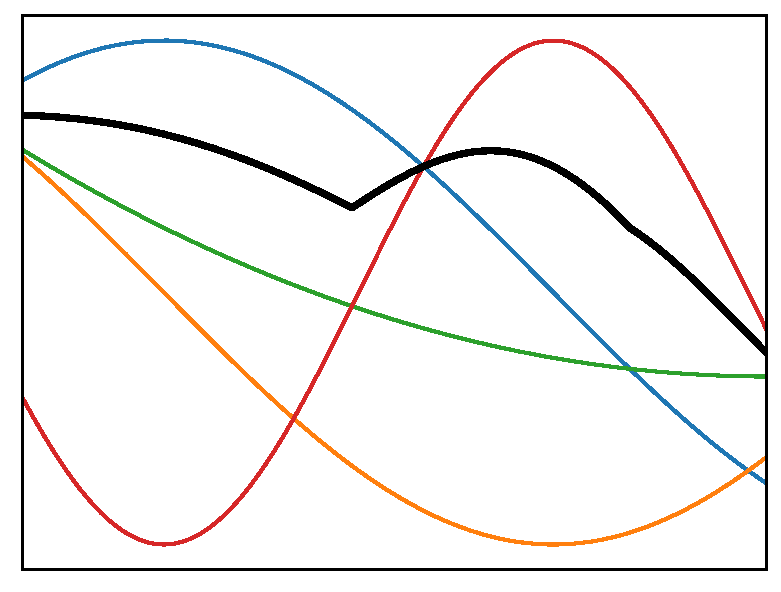
\includegraphics[width=\textwidth]{pictures/cvar.pdf}
         \caption{$J=\{3,4\}$}
         \label{fig:cvar}
     \end{subfigure}
        \caption{Order-Value functions for $J\subset\{1,2,3,4\}$.}
        \label{fig:ovexamples}
\end{figure}

 
% Chapter Template

\chapter{Chapter title}\label{Chapter2}
\lhead{Chapter 2. \emph{Order-Value Optimization}} 
\lipsum
\newpage
\section{Example of an algorithm}
\algorithm{alg:uvar}{Let $\delta>0$, $\sigma_{\min}>0$,
$\alpha\in(0,1)$, and $x^0 \in \R^n$ be given. Set $k\leftarrow 0$.}{
    \item\label{alg:uvar-step1} Choose $\sigma \geq \sigma_{\min}$ and initialize
    $\ell\leftarrow 1$.
    \begin{enumerate}
        \item\lipsum[1]
    \end{enumerate}
    \item\label{alg:uvar-step2} Compute $\xtrial$ as a solution of
    \begin{equation} \label{uvar-subpro}
      \Minimize \max_{i \in I(x^k,\delta)}
      \left\{ \nabla f_i(x^k)^T (x - x^k)\right\} +  \dfrac{\sigma}{2}\|x - x^k\|^2 .
    \end{equation}
}

 
\nolinenumbers

% Bibliografia
\backmatter
\nocite{*}
\lhead{\emph{Bibliography}}
\addcontentsline{toc}{chapter}{Bibliography}
\bibliographystyle{apalike}
\bibliography{bibliography}
\end{document}